\subsection{Sicherheitslücken bei bekannten Computer Herstellern}
Man sollte davon ausgehen können, dass die großen PC-Hersteller selbst am besten wissen müssten, wie hart der Markt in der Computerbranche umkämpft ist. Neben einer hohen Hardware-Qualität ist Kundenvertrauen immens wichtig. Zwei der weltweit bekanntesten und erfolgreichsten Computerhersteller \cite[vgl.]{pc_hersteller} haben den Faktor \textit{Vertrauen} nicht hinreichend erfüllt. Denn sowohl Lenovo als auch DELL haben das Vertrauen ihrer Kunden stark missbraucht. 

\subsubsection{Lenovo mit potentiellem Risiko}
%\subsubsection{Allgemeiner Ablauf}
Durch eine bereits vorinstallierte Software der Firma Superfish hat Lenovo versehentlich eine gravierende Sicherheitslücke auf einigen ihrer vertriebenen Notebookmodelle eingebaut. Dadurch wurde der Kunde einer zusätzlichen Gefahr eines erleichterten Hackerangriffes ausgesetzt.
%Mit der Superfish-Software beabsichtigte Lenovo, dem Nutzer gezielt personalisierte Werbung während des Surfens im Internet anzuzeigen. Um dies auch bei verschlüsselten Internetverbindungen (HTTPs) zu ermöglichen, wurde bei der Softwareinstallation auf den neuen Notebooks ein von Superfish selbst erstelltes Root-Zertifikat mit installiert. Der Kunde kaufte somit unwissentlich ein neues Notebook, auf dem ein bereits vor der Auslieferung manipuliertes Windows-Betriebssystem läuft. 
%Mit dem selbst signierten Root-Zertifikat wurden sichere (verschlüsselte) HTTPs-Verbindungen in Form einer Man-in-the-Middle Attacke aufgebrochen. Dadurch konnte sämtlicher Datenverkehr mitgelesen und  manipuliert werden. Im Fall von Lenovo geschah dies durch Einblendung von Werbung. 

%\subsubsection{Der Angriff und die benötigten Mittel}
Die Internetseite \url{www.golem.de} beschreibt die Idee und den Ablauf von den benutzerspezifischen Werbeeinblendungungen auf den Lenovo-Rechnern wie folgt: 
\begin{quote}
	\glqq Grundsätzlich ist die Idee von Superfish, dass das Programm Bilder auf Webseiten durchsucht und anhand von Algorithmen versucht zu erkennen, was sich darauf befindet. Auf Basis dessen werden dem Nutzer passende Shopping-Angebote als Werbebanner angezeigt. Geradezu zynisch wirkt die Beschreibung des Lenovo-Angestellten im Forum: Die Funktion diene dazu, Nutzern zu helfen, visuell Angebote für Produkte zu finden, bei denen sie Schwierigkeiten haben, sie mittels einer textbasierten Suchmaschine zu finden.\grqq \cite{superfish}
\end{quote}
Für die Umsetzung der Idee reichte es nicht, dass nur ein Programm von Superfish auf den Lenovo-Rechnern installiert wird. Zusätzlich benötigte Superfish unbedingt ein selbst signiertes Root-/Wurzel-Zertifikat auf dem System. Ohne dieses Zertifikat wäre es nicht möglich gewesen, auch in verschlüsselten Internetverbindungen (HTTPs-Verbindungen) den Suchalgorithmus anzuwenden, um anschließend personalisierte Werbung einzublenden. Mit dem eigenem Root-Zertifikat war Superfish in der Lage, für jede Verbindung, die zu einer HTTPs-Webseite aufgebaut wurde, ein eigenes, gefälschtes Zertifikat dynamisch zur Laufzeit zu erzeugen. Dieses wurde automatisch anerkannt, da bereits dem zugehörigen Wurzelzertifikat vertraut wurde. Weil Superfish sein Root-Zertifikat direkt im Windows-Zertifikatsspeicher installierte, wurde dieses nicht extra überprüft. Denn allen Zertifikaten, die sich im Windows-Zertifikatsspeicher befinden, wird automatisch das Vertrauen geschenkt. Der Anwender bekam dadurch nicht mit, dass keine direkte verschlüsselte Kommunikation zu dem eigentlichen Server, der die Webseite hostet, aufgebaut wurde. 
\begin{figure}[H]
	\centering
	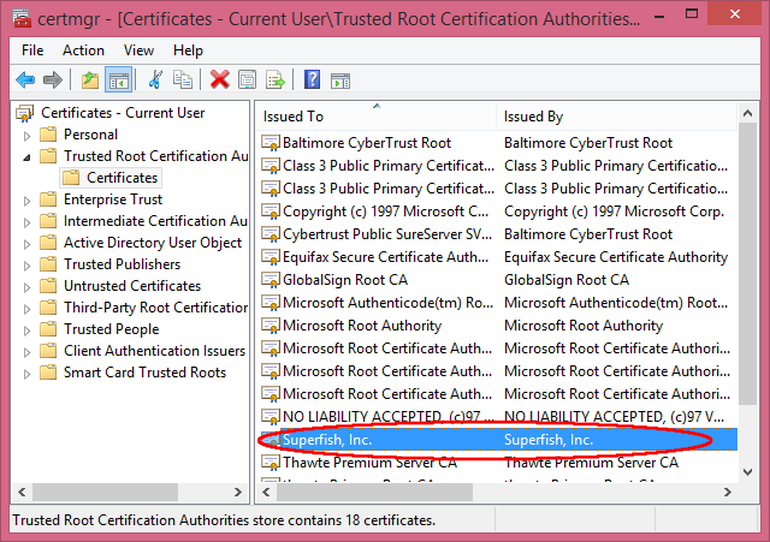
\includegraphics[width=.9\linewidth]{images/superfish.png}
	\caption{Superfish Root-Zertifikat im Windowszertifikatsspeicher, Quelle: \cite{superfish-bild}}
\end{figure}
\noindent %dadurch kein einrücken des Satzer, der nach dem Bild folgt
Weiterhin kam erschwerend hinzu, dass das Programm von Superfish für die Man-in-the-Middle Attacken ein schwaches Zertifikat nutzte. Das Root-Zertifikat verwendet für die digitale Signatur einen SHA-1 Hash-Alsgorithmus und für die asymmetrische Verschlüsselung ein 1024 Bit RSA-Verschlüsselungsverfahren. \cite[vgl.]{lenovo} Sowohl der SHA-1 Hash-Algorithmus als auch das RSA-Verschlüsselungsverfahren mit einer Schlüssellänge von 1024 Bit sind bereits erfolgreich geknackt worden und daher als unsicher einzustufen. \cite[vgl.]{sha-1,rsa}
Doch noch fataler als der Einsatz des unsicheren Hash-Algorithmus und des zu schwachen Verschlüsselungsfahrens, ist die Leichtigkeit der Entschlüsselung des privaten, geheimen Schlüssels. Robert Graham beschreibt in seinem Blog auf Errata Security eindrucksvoll, wie mit simplen Mitteln der Private Key exportiert und anschließend mit einer einfachen Wörterbuch-Attacke entschlüsselt werden konnte. \cite[vgl.]{certificate_ex}
Mittels des privaten Schlüssels kann jeder Angreifer, genau wie das Superfish-Programm, eigene, durch das Root-Zertifikat signierte, Zertifikate erzeugen und diese für bösartige Verwendungen nutzen. Somit bekommen die Anwender nicht mit, dass sie z. B. auf einer gefälschten Webseite surfen und ihre Daten ausspioniert oder manipuliert werden. Neben Zertifikaten für Webseiten, ist ein Hacker auch in der Lage, Zertifikate für kriminelle Software (z. B. Malware) zu erstellen und diese dem Nutzer als gutartig erscheinen zu lassen.  

\subsubsection{DELL mit ähnlichen Fehlern}
Der Computerhersteller DELL leistete sich einen ähnlich gravierenden Sicherheitsfehler wie sein Konkurrent Lenovo zuvor. Genau wie Lenovo hat DELL auch selbst signierte Root-Zertifikate auf einigen seiner Laptops installiert. Bei dem US-amerikanischen Hersteller sind es sogar zwei Root-Zertifikate. Sowohl das eDellRoot, als auch das DSDTestProvider Zertifikat wurden, genau wie das Superfish-Zertifikat, im Windows-Zertifikatsspeicher abgelegt. Beim Aufruf der allgemeinen Eigenschaften des eDellRoot-Zertifikats wird sogar ein Hinweis angezeigt, dass ein passender Private Key vorhanden ist. Joe Nord wendet in seinem Online-Blog die gleichen Vorgehensweisen zum Export und zur Entschlüsselung des DELL Private Keys an, wie Robert Graham beim Superfish Private Key. \cite[vgl.]{dell_joe_nord} 

\begin{figure}[H]
	\centering
	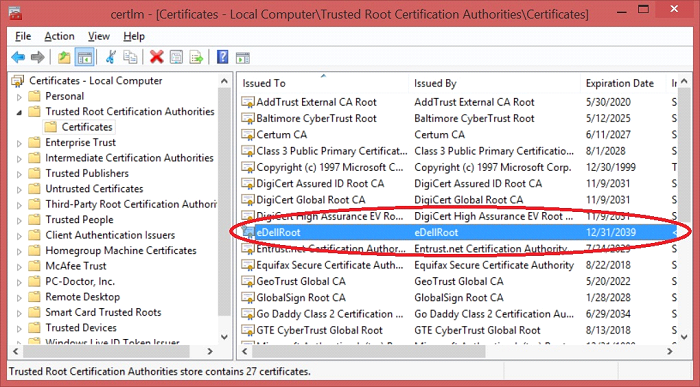
\includegraphics[width=.7\linewidth]{images/eDELLRoot.png}
	\caption{Ausschnitt aus Windowszertifikatsspeicher mit installiertem eDELLRoot Zertifikat, Quelle: \cite{dell}}
\end{figure}
	
\begin{figure}[H]
	\centering
	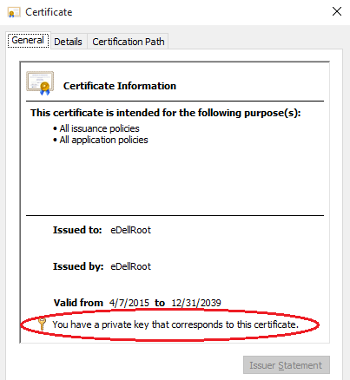
\includegraphics[width=.4\linewidth]{images/cert_eDELLRoot.png}
	\caption{Eigenschaftsansicht von eDELLRoot Zertifikat mit Hinweis auf Private Key, Quelle: \cite{dell_joe_nord}}
\end{figure}
\noindent
Angreifer mit dem privaten DELL Schlüssel haben die gleichen Angriffsmöglichkeiten auf infizierte DELL Geräte, wie Angreifer mit dem Superfish Private Key auf infizierte Lenovo Geräte.
Beide DELL Zertifikate wurden durch Software installiert, das eDellRoot Zertifikat mit dem Dell Foundation Services Programm und das DSDTestProvider Zertifikat mit der Dell System Detect Software. 
Sie sollen, laut DELL, für einfacheren Support dienen. 
DELL hat auf seiner Webseite folgende Stellungnahme publiziert: 
\begin{quote}
	\glqq[...] Das Zertifikat eDellRoot wurde zusammen mit unserer Anwendung Dell Foundation Services installiert und wird zur Unterstützung einer besseren, schnelleren und einfacheren Support-Erfahrung für unsere Kunden verwendet. Das Zertifikat ist keine Schadsoftware oder Adware. Es war ursprünglich dazu gedacht, die Service-Tag-Nummer des Systems an den Onlinesupport von Dell zu übermitteln, damit wir schnell das Computermodell identifizieren und unseren Kunden so einen unkomplizierteren und schnelleren Service bieten können. Das Zertifikat wird nicht zum Sammeln persönlicher Kundendaten verwendet. Bitte beachten Sie, dass sich das Zertifikat nicht von selbst neu installiert, nachdem es mit dem empfohlenen Dell Prozess ordnungsgemäß entfernt wurde.\\
	Wenn wir eDellRoot kennen, können wir uns auf alle unsere Anwendungen konzentrieren, die auf Dell PCs geladen werden. Wir können bestätigen, dass keine weiteren Root-Zertifikate auf dem werkseitig installierten Image installiert wurden. Wir haben jedoch herausgefunden, dass die Anwendung Dell System Detect  und das dazugehörige Root-Zertifikat DSDTestProvider ähnliche Eigenschaften hat wie eDellRoot. Im Fall von Dell System Detect lädt der Kunde die Software proaktiv herunter, um mit der Webseite vom Dell Support zu interagieren. Dadurch können wir eine bessere und individuell abgestimmte Support-Erfahrung anbieten. Wie eDellRoot auch wurde das fragliche Support-Zertifikat entwickelt, um unseren Kunden einen schnelleren und einfacheren Support zu bieten. Die Vorteile sind jedoch auf die Kunden beschränkt, die die Funktion zur Produkterkennung auf unserer Support-Webseite zwischen dem 20. Oktober und dem 24. November 2015 genutzt haben. Die Anwendung wurde von der Dell Support-Webseite sofort entfernt und es steht ab sofort eine neue Anwendung ohne das Zertifikat zur Verfügung. Wir unterstützen proaktiv ein Software-Update, um das Problem anzugehen und haben im Folgenden Anweisungen zum Entfernen des Zertifikats bereitgestellt.\grqq \cite{dell}
\end{quote}
Mit dieser Aussage hat DELL offiziell bestätigt, eigene Zertifikate auf Nutzer-Endsystemen installiert zu haben. Das eDellRoot wurde augenscheinlich bereits vor Auslieferung auf den Geräten installiert und das DSDTestProvider erst nachträglich durch Installation und Verwendung des DELL Support-Programms. Durch das DELL-Statement fällt auf, dass das eDellRoot Zertifikat sich eventuell erneut installieren kann, wenn es nicht mit spezieller DELL Software bzw. geeignetem DELL Prozess richtig deinstalliert wurde. 
\begin{quote}
	\glqq[...] Bitte beachten Sie, dass sich das Zertifikat nicht von selbst neu installiert, nachdem es mit dem empfohlenen Dell Prozess ordnungsgemäß entfernt wurde.\grqq \cite{dell}
\end{quote}
Die Ursachen für eine eventuelle Neuinstallation des DELL Zertifikats sind im nachfolgenden Kapitel \ref{sub:schutz} \nameref{sub:schutz} beschrieben.